
\section{INTRODUCTION} 
During the latest stage of structure formation, the universe gave birth to
non-linear, hierarchical structures known as galaxy clusters. 
These clusters, made up of dark matter, galaxies and hot gas,
are constantly accreting, merging and evolving with their
environments. Bright galaxies that belong to a galaxy cluster or group, in 
particular, highlight the overdensities of the underlying dark matter (DM) 
distribution. 

% Peaks, summary statistics 
% Modeling galaxy clusters - distributions, peaks, centroids 

In these high density regions of the clusters, the rates of particle
interactions can be enhanced, including the long-suspected self-interaction of DM
particles (hereafter, SIDM). 
Many papers have used the DM density peaks to give constraints on 
the self-interaction cross
sections of dark matter (\citealt{Markevitch2004}, \citealt{Bradac2006b}, Mertel , Dawson, Jee etc.). 

% Why we want to compare galaxies with the DM distribution? 

% What are the observational methods for summarizing dark matter distribution?
Weak and strong lensing are the most reliable methods for mapping the dark 
matter distribution in a galaxy cluster. 
Common to all the methods are the estimation of the density peaks. 


% What are the methods for summarizing the galaxy distribution?



We quantify the bias and uncertainty associated with the one-point summary
statistic for summarizing the physical state of a galaxy cluster. 
Commonly used one-point statistic of galaxy clusters include:
1) papers reported using centroids but did not state what centroid that they
used 
2) papers used center of mass 
3) papers that used peaks \citep{Robertson2016} 
% What are the reported offsets?
Offsets between different statistical measures of the galaxy and the DM
population are not going to be zero.
% Miscentering ?! want to capture the dominant component of the cluster 
% You only have one center when there is only ONE component 

Uncertainties affect the conclusion for the computation the hypothesis test / parameter
estimation
Previous work on quantifying galaxy-DM offsets included  
What centroids they have used

Physical motivation for using the galaxy density peak 
Observation footprints 

Under the assumed Lambda Cold Dark Matter cosmology, it is unclear 
that how large the distribution offset $\Delta \vec{s}$ should be. 
% Why use simulation data to study the populations? 
Other complications for studying galaxy clusters arise from observation
limitations. There is not a lot of information that can help constrain the  
line-of-sight distance of different components of a cluster. 


% Goals of the paper
With the advent of large-scale sky surveys, 
the number of identified galaxy clusters is growing quickly. 
Existing catalogs such as the Abell catalog also contain
at least 4000 clusters with at least 30 members. 
The future Large Synoptic Sky Survey alone will identify over a hundred thousand galaxy
clusters (CITE). It is important to verify the uncertainties associated with common
summary statistics for studying galaxy clusters. Considering the large quantity
of data, it is hard to use methods that require manual tuning if we want to
obtain consistent statistics from the samples.

In this paper, we 
1) extract realistic observables from the Illustris simulation for
comparison with observations, 2) explore the pros and cons of the different statistic for 
summarizing the member galaxy population of a galaxy cluster, 3)	
give estimates for the offsets between the summary statistics of the galaxy  
population and the DM population, which we call 
\begin{equation}
	\Delta s \equiv \vec{s}_{\rm gal} - \vec{s}_{\rm DM}.
\end{equation}
where $\bf{s}_{gal}$ and $\bf{s}_{DM}$ are the two dimensional (2D) spatial
locations of the summary statistic of the galaxy population, and the density
peak of DM respectively. 
Finally, we provide the distribution and investigate which quantities that are most
correlated with of $\Delta s$.

\begin{figure*}
	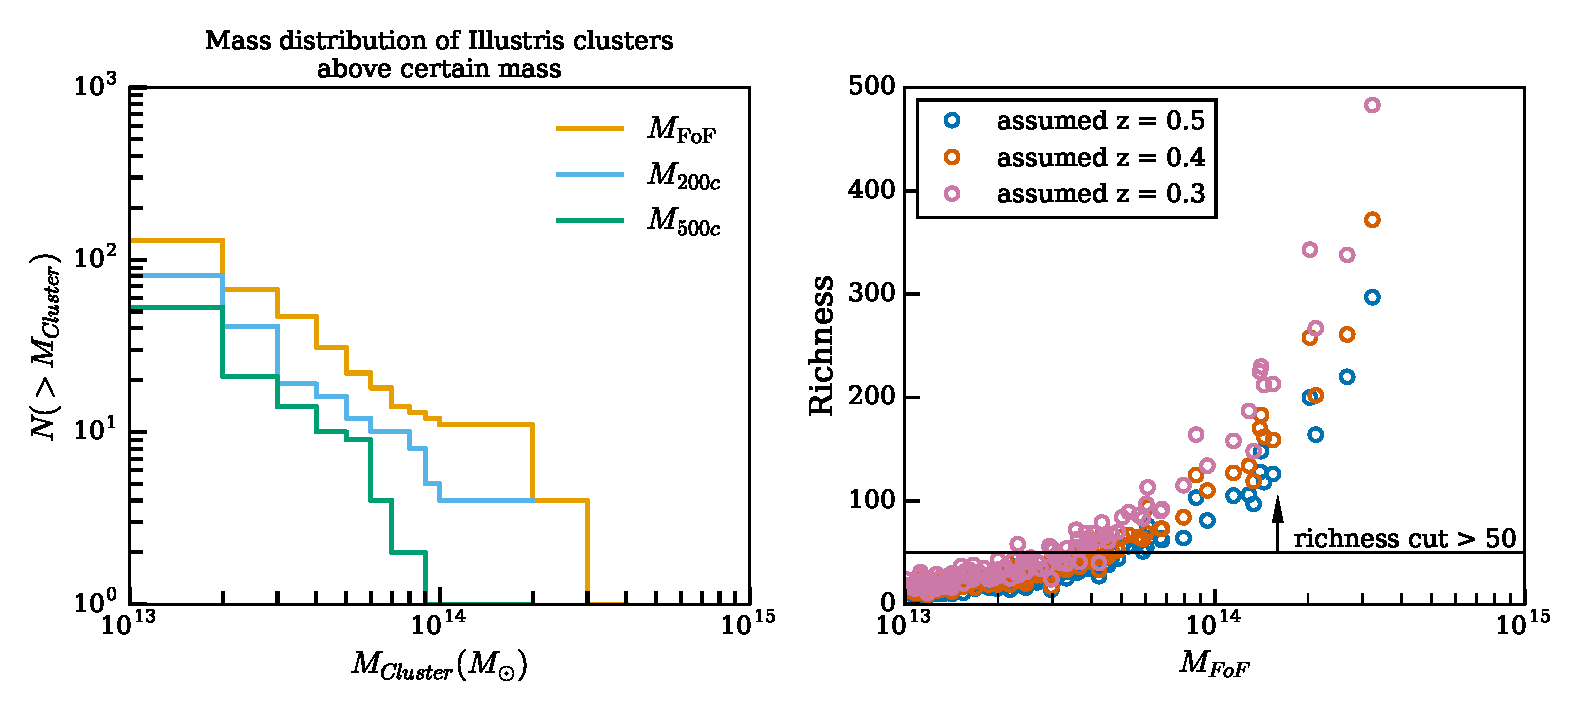
\includegraphics[width=\linewidth]{fig1_mass_richness.eps}
	\caption{ {\bf Left figure:} Mass distribution of the group / cluster sized 
		DM halos for different halo selection schemes. Mass estimates obtained by the
		FOF algorithm are labeled as  M$_{\text{FoF}}$.
		Masses centered on the most bound particle within a radius those the 
		average density is 200 or 500 times the critical density of the universe are 
		labeled as M$_{200c}$ and M$_{500c}$ respectively. 
		Discrepancies between the different
		measures of mass of the clusters indicate the presence of spatially
		separated substructures for the clusters (See Fig. 
		\ref{fig:select_peak_visualization}). {\bf Right figure:} 
		Mass-richness relationship of galaxy clusters and groups with 
		$M_{\rm FoF} > 10^{13} M_{\sun}$ . We require clusters to have more than 50 member 
		galaxies that are above observation limit, i.e. apparent $i \leq 24.4$ when 
		we assume a cosmological redshift
of $z=0.3$, as shown by the richness cut. A total of 43 clusters have 
survived this cut. \label{fig:mass_richness}}
\end{figure*}

% Basic setup 
The organization of this paper is as follows:
In section \ref{sec:illustris_sim}, we will describe the physical properties of 
the products of the Illustris
simulation (\citealt{Vogelsberger2014}, \citealt{Genel2014a}), 
and the selection criteria that we have employed to ensure that the
quantities that we examine resemble observables but without noise and
systematics from observations. 
Then in section \ref{sec:methods}, 
we will describe the methods for computing various 
one-point statistics of the spatial distribution of galaxies how we prepare our dark
matter spatial data to resemble convergence maps. We will show the comparison
of the different summary statistics before we show the main results
in section \ref{sec:results}. Finally, we will discuss the implications of our
results and compare it to other simulation and observations.

Our analysis makes use of the same flat Lambda Cold Dark Matter ($\Lambda$CDM) cosmology
as the Illustris simulation. The relevant cosmological parameters are
$\Omega_\Lambda = 0.7274, \Omega_m = 0.2726$, and $H_0 = 70.4$
km~s$^{-1}$~Mpc$^{-1}$.

\section{THE ILLUSTRIS SIMULATION DATA} 
\label{sec:illustris_sim}


The Illustris simulation that we made use of contains some of the most
realistic, simulated galaxies to date. We obtained our data from 
snapshot number 135 of the Illustris-1 simulation ($z=0$). The Illustris-1
simulation has the highest particle resolution and has incorporated the most 
comprehensive baryonic physics among the different Illustris simulation suites. 
The sophisticated galaxy formation model in Illustris-1 
 includes star formation rate, stellar evolution due to
environmental effects and supernovae feedback etc. The physics of stellar
evolution were solved using a moving mesh code {\bf \texttt{AREPO}} \citep{Springel2010}.
This simulation formalism accounts for the environment effects of a cluster to the
evolution of galaxies. The galaxies were statistically consistent
with the Sloan Digital Sky Survey data
\citet{Vogelsberger2014}. Since the profile of the galaxies clusters were not
provided by known, symmetrical parametric forms, we can study 
how asymmetry in the cluster profile affects the estimate of our summary 
statistic. Thus, this data allows us to examine cluster galaxies
in a realistic, yet noise-free way.

The catalog that maps particles to the halo of a certain cluster was created by
the {\bf \texttt{Subfind}} algorithm.
Galaxy data: 
The friends-of-friends (FOF) finder (CITE properly: Davis et al. 1985) was used to identify
dark matter structures. These galaxy-size halos are also referred to as
subhalos, the dark matter host of what we refer to as galaxies in Illustris-1. 

Data matter data:
While {\bf \texttt{Subfind}} was used to identify the affinity of particles 

The observation bands available in the Illustris data include the $u, g, r, i,
z$ bands. 

\begin{figure}
	\centering
	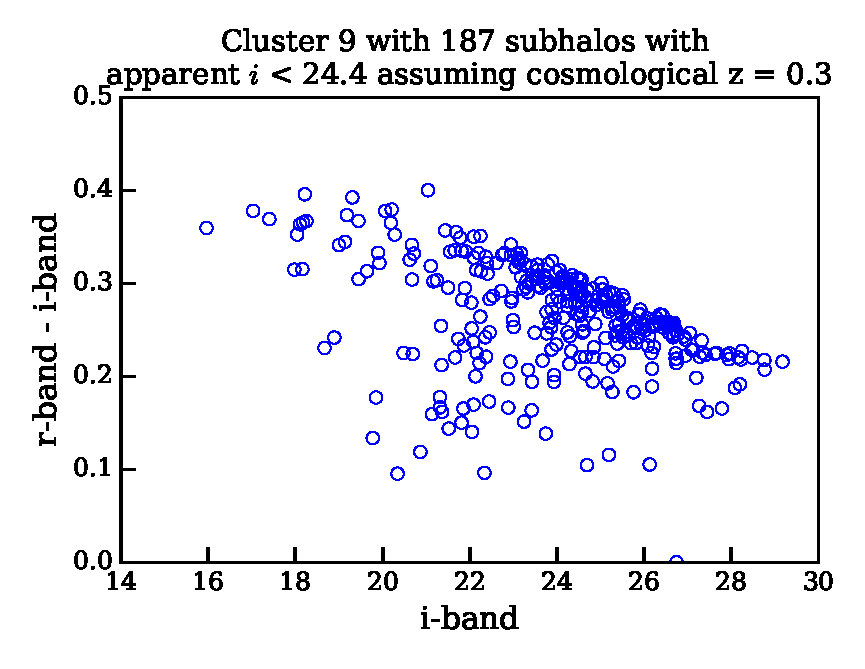
\includegraphics[width=\linewidth]{fig2_color_magnitude_diagram9.eps}
	\caption{Color-magnitude diagram of one of the galaxy clusters that is selected for 
		analysis. This cluster is the 9th most massive. 
		The apparent magnitude is calculated assuming that 
		the cosmological redshift (distance) is $z = 0.3$. 
		We can see a clear overdense region that corresponds to a red-sequence.
		The color-magnitude diagrams of the other clusters can be found in the
		Jupyter notebook at \href{https://github.com/karenyyng/galaxy_DM_offset/blob/master/code/analyses/fig2_color_magnitude_diagram.ipynb}{https://goo.gl/TJmI6s}.
		\label{fig:color_magnitude_diagram}
	} 
\end{figure}
For our results, we make use of galaxy clusters / groups 
that have at least 50 member galaxies after this magnitude cut in the $i$ band. 
This is because of the relatively large statistical uncertainty from if we try
to analyze clusters with less than 50 member galaxies. 



% LSST goes as deep as 27.5

\subsubsection{Cluster properties}
\label{subsubsec:cluster_properties}

\subsection{Relaxedness of the clusters}

Clusters undergo merger activities in the time scale of million of years. 
Observations can only provide snapshots of the state of a cluster. 
This info is also hard to retrieve from simulations across different saved
states.
We quantify the state of the cluster by providing several quantitative
definitions of non-relaxedness and see how they correlate with $\Delta s$.
Some definitions of non-relaxedness referred by the simulation community
include:
\begin{itemize}
	\item ratio of mass outside the dominant dark matter halo over the total mass
		of the galaxy cluster 
	\item distance between the most bound particle from the center of mass as a
		function of $R_{200c}$.
\end{itemize}
While we try to provide more observation oriented quantities as we would
discuss in the method section \ref{subsubsec:KDE}. 


\subsection{Selection of the field of view}
\label{sec:FOV}

\begin{table*}
\begin{center}
\begin{minipage}{180mm} 
	\caption{ Selection criteria for stellar subhalos (member galaxies) for each
		cluster / group 
\label{tab:member_galaxy_selections}} 
	\begin{tabular}{@{}lcccc@{}}
\hline 
Data &  Selection strategy  & Sensitivity & Relevant section  \\ \hline
Field of view (FOV) & FOF halo finder& comparable to FOV of the Subaru
Suprime camera &   \\ 
Observed filter & $i$-band & consistent over the redder $r, i, z$ bands &   \\ 
Cluster richness  & $i \leq 24.4$ and $z = 0.3$  & sensitive to
the assumed cosmological redshift of cluster and &    \\ 
& & the assumed limiting magnitude of telescope &   \\
Two-dimensional projections & even HealPix samples over half a sphere &
discussed as results  & \\  
\hline
\end{tabular} 
\label{tab:selection_criteria} 
\footnotesize{
}
\end{minipage}
\end{center} 
\end{table*}

As a default output from the Illustris simulation, subhalos and particles of
each galaxy cluster and group are identified by the halo finder
(CITE). We make use of the member particle / subhalo identification as our
default volume selection scheme for each cluster / group.
We understand that this choice of volume selection can be more ideal than
observational conditions. We make use of this volume selection scheme
for baseline comparisons. 

Furthermore, assuming a conservative line-of-sight (los) distance 
, i.e. cosmological redshift, of $z = 0.4$, 
the projected extent for most of the Illustris galaxy clusters and groups, 
fits inside the field of view of telescopes, such as the Subaru Suprime Camera,
which covers a physical area of $\sim 9$ Mpc $\times 7$ Mpc. 
Halo and FoF finding is described in \citep{Vogelsberger2014}.

\subsubsection{Spatial Projections}
The summary statistics are computed all based on 2D matter projections of the
spatial location.
In order to represent the projection uncertainty, we sample the projections evenly
by using HealPy (CITE), which is a Python wrapper for HealPix (CITE).
The viewing angles of the projections are defined by an elevation angle
$\xi$ and an azimuthal angle $\phi$. 
The number of projections that we employed is FILL IN A NUMBER.

\begin{table*}
\begin{center}
\begin{minipage}{180mm} 
	\caption{Comparison between various methods for estimating the one-point
		statistics of the galaxies of a cluster 
\label{tab:centroid_comparison}} 
	\begin{tabular}{@{}lccccc@{}}
\hline 
Method &  One-point statistic & Sensitivity to biases & Uncertainty  & Relevant
section & Comment  \\ \hline
Centroid & 2D spatial averages & High & Low & \\
Shrinking aperture & proxy for density peak & Higher sensitivity to substructures & Medium
& \\
Peak finding from KDE & density peak & Lower sensitivity to substructures &
Higher & \\
Brightest cluster galaxy & & Sensitive to foreground contaminants & \\ 
Most bound particle & bottom of gravitational potential well &  & 
&  \\
\hline
\end{tabular} 
\label{tab:summary_stat_info} 
\end{minipage}
\end{center} 
\end{table*}
\subsection{Properties of galaxies in clusters}
\subsubsection{Galaxy weights}
\label{subsubsec:galaxy_weights}
Not all galaxies are created equal, so they should not be considered with equal
importance for peak identification, which requires summing the
the mass proxy of different galaxies. Galaxies reside in host halos with different masses and 
contain different stellar masses. The brightness of galaxies in a cluster are 
also affected by the cluster environments.
For example, the star formation rates of cluster galaxies are known to be 
suppressed by the high concentration of intracluster medium. (CITE)
One of the most common weighting schemes employed for galaxy data is to weight
by the luminosity in a particular band.

\section{METHODS}\label{sec:methods}

There are many reasonable models for summarizing the overall spatial
distribution of cluster components. Each method has different uncertainties.
Our goal here is to find the  
not to identify galaxies as parts of subcluster components,
but to find the location where we expect to see the highest mass density of the
DM.

Reasonable models fall under several categories, 1) mixture models, 2) basis function
expansions, such as wavelet methods and 3) non-parametric estimations 
such as a kernel density estimation, or hierarchical clustering. 
Not only do the performance of the 
first two methods depend heavily on model parameters, 
the data fit also depend quite strongly on the functional form of 
the underlying mixture model / wavelet basis. Often times, 
the mixture models and wavelet bases 
carry strong symmetry assumptions that may not be valid for spatial modeling of 
hierarchically formed galaxy clusters. 
This is because galaxy clusters have substructures over a wide range of length
scales, from galaxy scales of hundreds of pc to fraction of a Mpc. 
The symmetry assumption will bias the estimate of the point estimate that we
are after for non-symmetric clusters.

Well known tradeoff Bias-variance tradeoff

Goal: to identify the ``center'' of the light distribution. Here the adopted 
tracers for the light distribution are the member galaxies of the cluster 
and groups.

We do not claim that point estimates are sufficient statistics for
best representing the physical states of galaxy clusters nor the effect of
self-interacting dark matter. However, we try to understand the impact of the
different choices of point estimates on the estimate of $\Delta s$. 
We compare four ways to identify the light/galaxy centers:
\begin{enumerate}
\item Centroids
\item KDE + peak finder
\item Shrinking aperture method
\item Brightest cluster galaxy (BCG)

\end{enumerate}

We try to avoid any manual methods for identifying peaks for
reproducibility and comparison purposes. Since all the methods listed in this
paper are automated, it is possible for other studies to reuse our code for 
comparisons. 
There are a number of decisions ($\sim [TODO] ADD NUMBER$) that one needs to make to 
determine the summary statistics. We will try to address the sensitivity of the offset
due to each decision. 
Furthermore, a major advantage for automation is that it allows us  
to scale up our analysis by applying
the same methods across the different snapshots of the Illustris simulations to
examine the variability of $\Delta s$ across time. 


\subsubsection{Centroids or center of mass}
\label{Unweighted}
We follow the usual definition of spatial centroid as 
\begin{equation}
	\bar{\bf x} = \frac{1}{n} \sum_i \vec{x}_i. 
\end{equation}
While the weighted centroids are just: 
\begin{equation}
	\bar{\bf x}_w = \frac{\sum_i w_i \vec{x}_i}{\sum_i w_i},
\end{equation}
for each spatial dimension and the weights $w_i$ for the $i$-th galaxy
is described in section.
Centroids can be biased 1) by subcomponents from merging activities yet the
centroid estimate do not provide explicit evidence for ongoing merger or 
accretion, 2) by the field of view.

\subsubsection{Cross-validated Kernel Density Estimation (KDE) and the peak finder} 
\label{subsubsec:KDE}
We employed a KDE algorithm to infer a smooth density distribution of the
sparse galaxies.
It is known that the choice of the functional form of the smoothing kernel does
not dominate the density estimate $\hat{f}$ as long as the chosen kernel is
smooth (CITE). Instead we focus our effort to use cross-validation to obtain 
the optimal 2D smoothing
bandwidth matrix for each cluster ($\Hmat$) for our 2D Gaussian kernel. 
\begin{align}
	\hat{f}(\chi; \Hmat) &= \frac{1}{n} \frac{1}{(2\pi)^{d/2}|\Hmat|^{1/2}}
	\sum_{i=1}^n \exp((\chi-{\bf x}_i)^T H^{-1} (\chi-{\bf x}_i)),
\end{align}
where the dimensionality is $d=2$ for our projected quantities,
$X$ represents the uniform grid points for evaluation, and 
$\bf{x}_i$ contains the spatial coordinates for each of the identified member 
galaxies that survived our brightness cut.

Specifically, we made use of the KDE function in
the statistical package {\bf \texttt{ks}} (CITE Duong) in the R statistical 
computing environment (CITE R Core Team 2014). 
Cross validation eliminates free parameters in the KDE and minimizes
the asymptotic mean-integrated squared error (AMISE) for a best fit to the
data. Although the smoothed cross validation technique takes $O(n^3)$
(DOUBLECHECK) computational requirement, the number of cluster galaxies are
small enough for this method to finish quickly. 

After obtaining the KDE estimate, we employed both a first and second-order  
finite differencing algorithm to find the local maxima.  
The local maxima were then sorted according to the KDE density.  


% TODO: talk about the 

Spatial location and the density of the subdominant peaks are also stored.
We investigated if the presence of subdominant peaks are correlated with
$\Delta s$. 

\subsubsection{Shrinking aperture}
Another popular method among astronomers for finding the peak of a spatial
distribution include what we call a shrinking aperture method.
We test if the shrinking aperture method is able to reliably recover the highest 
peak.
This method is dependent on the initial diameter and the initial center 
location of the aperture.
This method does not evaluate if the cluster is made up of
several components.
The estimate using the shrinking aperture algorithm can be biased by
substructures. The only way to inform the algorithm about substructures would
be to introduce another parameter to restrict the center of the aperture, or to
partition the data.
Furthermore, the convergence rate for this iterative algorithm is not
analytical and is dependent on the data. We present the
convergence criteria for reference. 
We note that the exact implementation may result in different performances.
\begin{algorithm}
	\caption{Shrinking aperture algorithm. See code at (TODO: ADD LINK TO CODE ON
	GITHUB)}
	\KwData{subhalo that satisfy cuts as a galaxy}
	 \hrulefill \\

	 initial aperture centroid = mean galaxy location in each spatial dimension\\
 	distance array = euclidean distance between initial aperture center and galaxy
	location \\
 	aperture radius = 90th percentile of the distance array\\ 
	\While{ (newCenterDist - oldCenterDist) / oldCenterDist $\geq$ 2e-2}{
 		new data array = old data array within apert\\
 		newCenter = mean value of new data along each spatial dimension 
	}   \hrulefill
 \end{algorithm}
 See [TODO] LINK to BitBucket code repository for the Python implementation
 along with the unit test.


\subsubsection{Brightest Cluster Galaxies (BCG)}
The BCGs are formed by the merger of many smaller
galaxies. The galaxy-cannibalism makes BCGs typically brighter than the rest the 
cluster galaxy population by several orders of magnitude. (CITE?)
However, star formation can result
in galaxies brighter in the bluer photometric bands.
To avoid star formation from biasing our algorithm for identifying the
BCG, we find at the brightest galaxies in redder bands i.e. the $r, i, z$
bands and found that they give consistent results for all selected clusters. 
The band in which we picked the BCG for presentation is the $i$-band. 

\begin{figure*}
	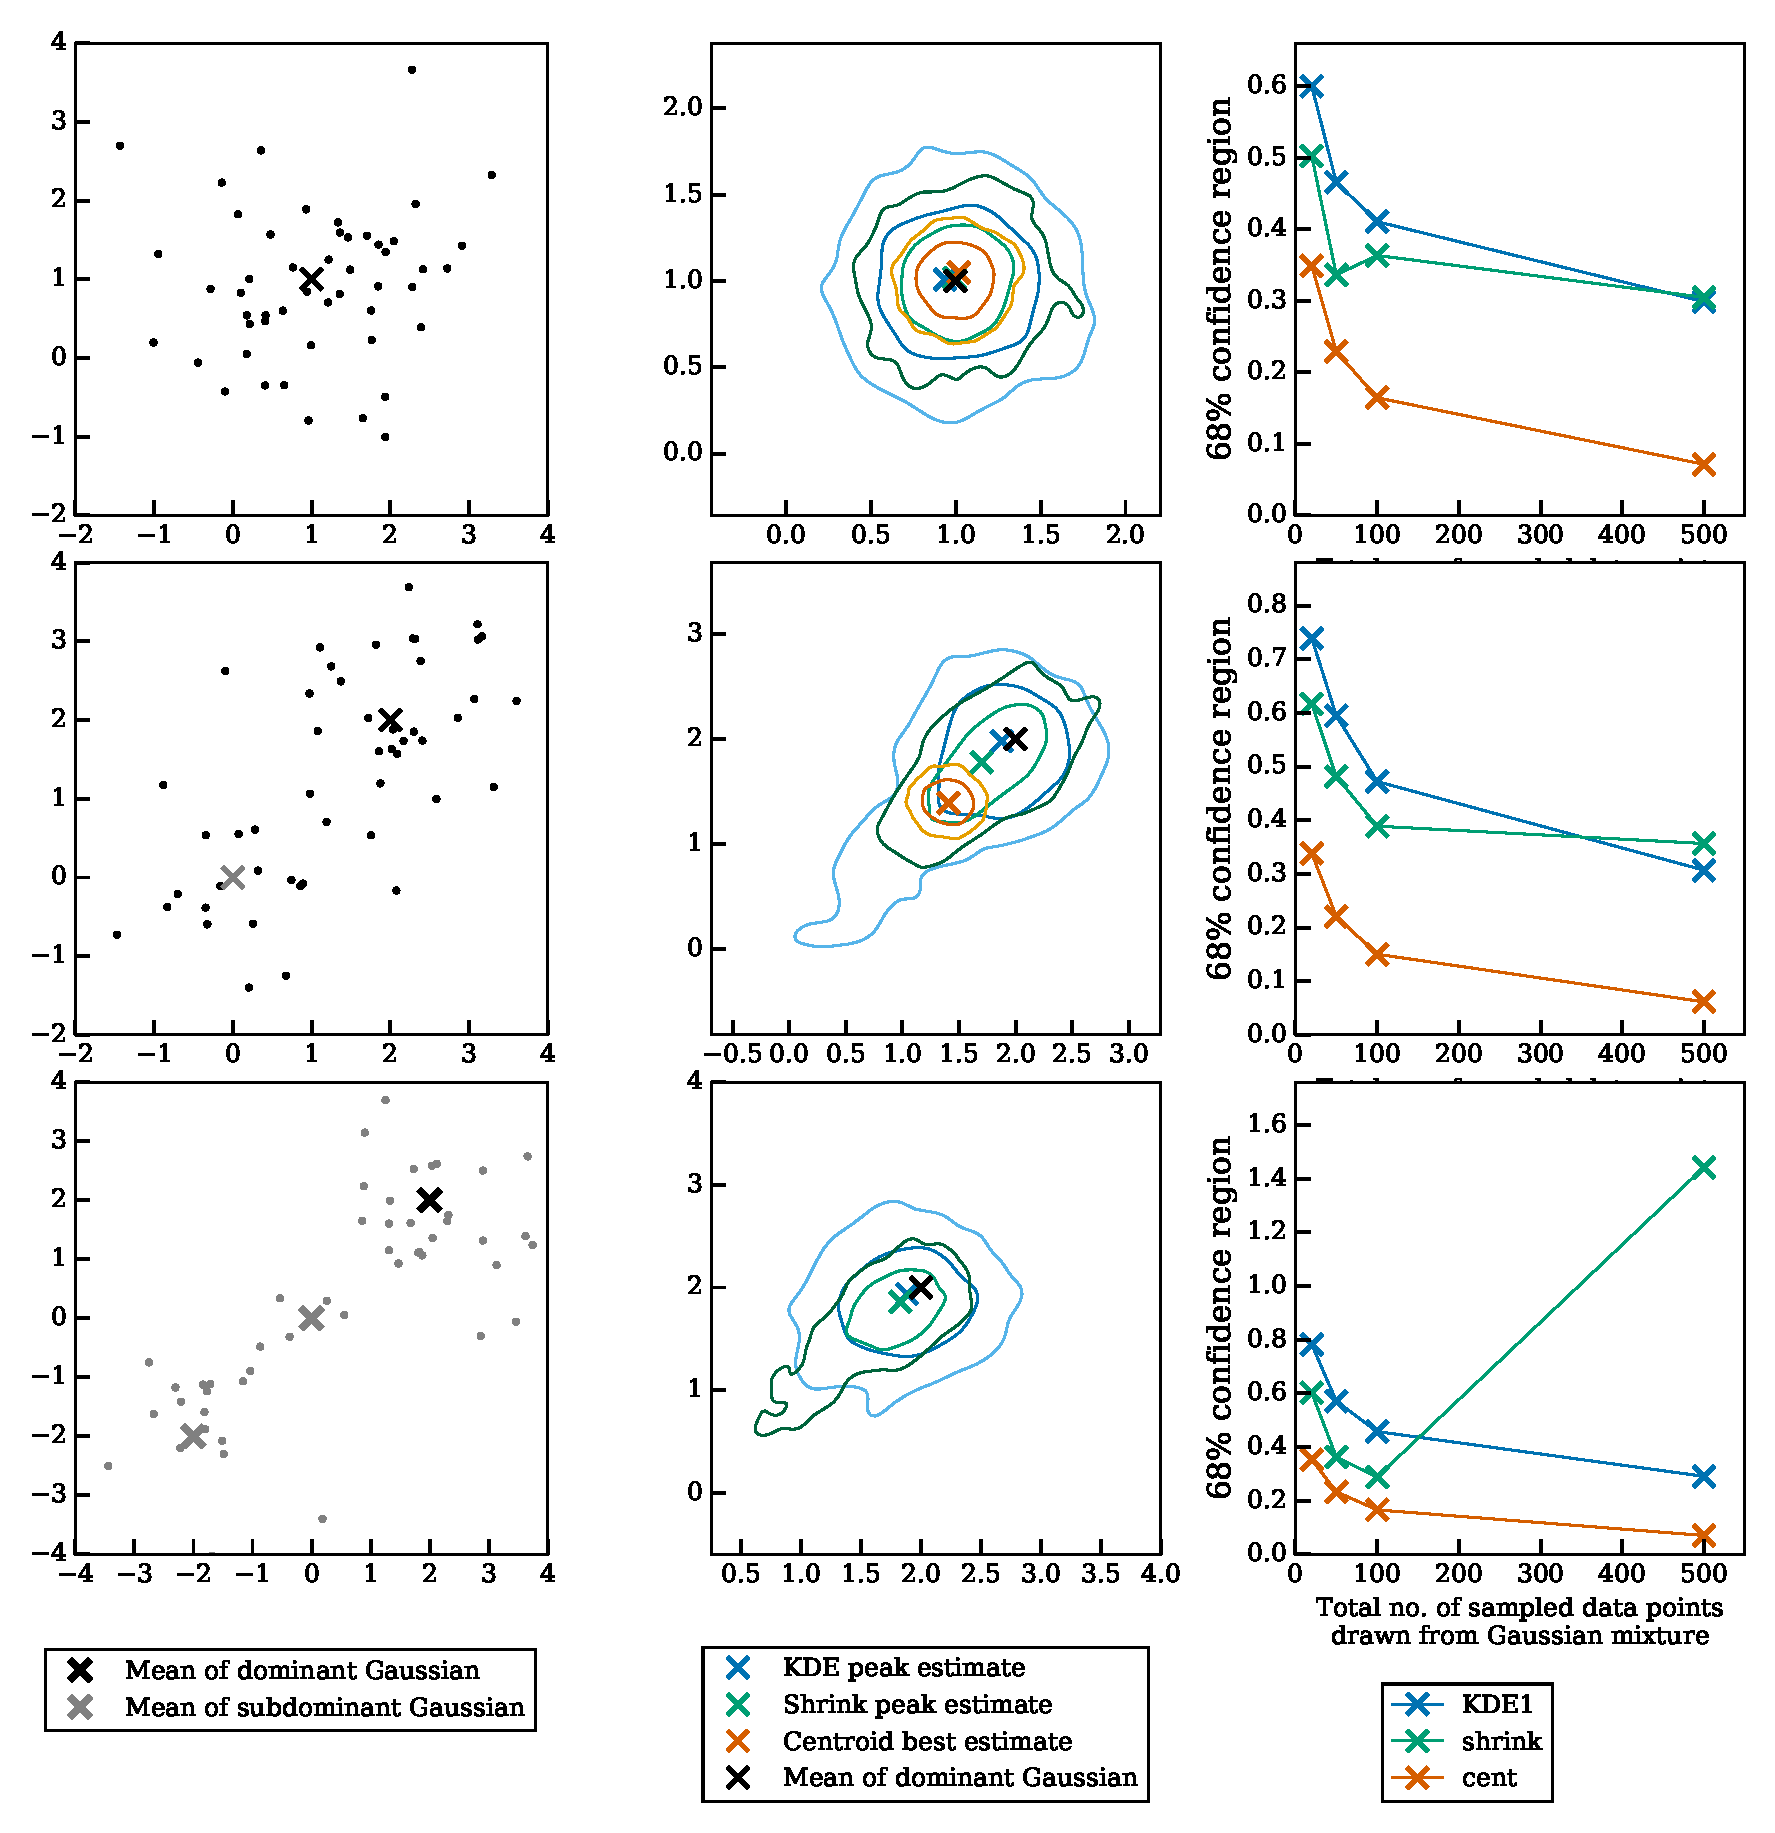
\includegraphics[width=.95\linewidth]{fig3_toy_data_mixtures.eps}
	\caption{[TODO] ADD LEGEND TO THE PLOT. 
		Comparison of peak finding performances of different methods. Panels
		from the top row contain data drawn from a single Gaussian mixture. The
	second row panels contain data from two Gaussian mixtures. 
		\label{fig:toy_data_mixtures}}
\end{figure*}



\subsection{Comparison of the methods from test data}
In order to examine the performance of commonly used point-estimates of the
distribution of the galaxy data, we test them on data drawn from Gaussian mixtures with
known mean and variance. (See \ref{fig:toy_data_mixtures})\\
We compare the properties and performance of each of the
methods for finding the peaks of the galaxy and dark matter. 
The main factors that affect the performance of the methods depend heavily on
statistical fluctuations of the drawn data. Namely, the performance of each
method depends on: 1) the
actual spatial distribution of the data, in this case, the parameters of the
gaussian mixtures that we chose, 2) the number of data points that we draw from 
the distribution.
Due to the statistical nature of the data, it is not enough to just
compare the performance by applying each method for one realization of the
data. We also provide the 68\% and the 95\% confidence regions from the
different methods for different Monte Carlo realizations.
In general, the 


The details and implementation can be found in our Bitbucket Git repository.



\subsection{Modeling the DM map in Illustris-1 and the lensing kernel}
The most established method of inferring the projected dark matter spatial 
distribution from observations is through gravitational lensing.
It works by detecting subtle image distortions of background galaxies due to
the foreground dark matter. The resolution of the inferred map therefore 
depends on the properties of the galaxies, such as the projected number density, 
intrinsic ellipticities and morphology etc.
To achieve a sufficient signal-to-noise ratio for lensing, 
Hoag et al. (in prep) has performed simulation for inferring the optimal size
for a Gaussian smoothing kernel. 
In the strong lensing regime, Hoag et al. found a resolution of 11 arcseconds
can best maximize the fit. This kernel translates to a physical size of [TODO]
kpc assuming a cosmological redshift of [TODO] $z = 0.3$.
To infer the 2D projected density from Illustris-1, 
we constructed (smoothed) histograms of the DM
particles of each selected galaxy cluster. 
Physically, the 2D histogram of the dark matter of each cluster 
is analogous to a convergence map from a lensing analysis. 
We further show results after convolving the histograms with different kernel
size.   


% - [  ] Add the equation calculating a lensing kernel due to S/N constraint 
% apropos conversation with Marusa and Austin 's 


\subsection{Finding offsets} 
We computed the projected offsets between the galaxy density peaks inferred from the
cross-validated KDE peaks of the galaxy data and the maximum DM density peaks.

% It is possible to also  





\section{RESULTS} 
\label{sec:results}



\subsection{Visual inspection of galaxy clusters}
From the high resolution visualization of the DM maps (2 kpc histograms) in 
\ref{fig:select_peak_visualization}, we can tell that some clusters clearly
possess multiple subclusters. However, there are also several clusters with
only one main component that has several peaks (galaxies) in the central region. 
This illustrates why finding a `center' or peak of a cluster is an ill-defined 
notion. Furthermore, we show a lower-resolution visualization of the DM surface
map in Fig. [TODO] compared to the higher resolution map, we can see a clear
shift in the peak location. This illustrates that peak / center finding is also
subject to noise from the data.




\begin{figure*} 
	\centering
	% 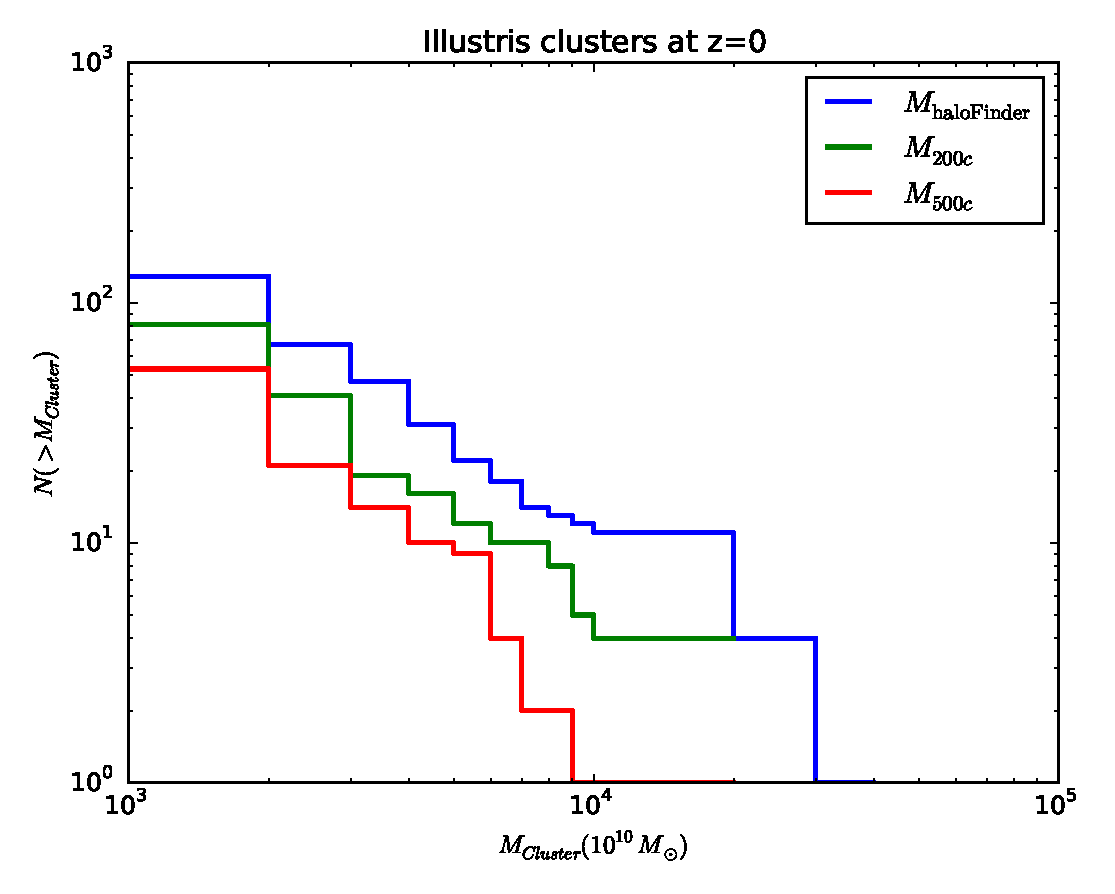
\includegraphics[width=\linewidth]{clusterMassDist.eps}
	% 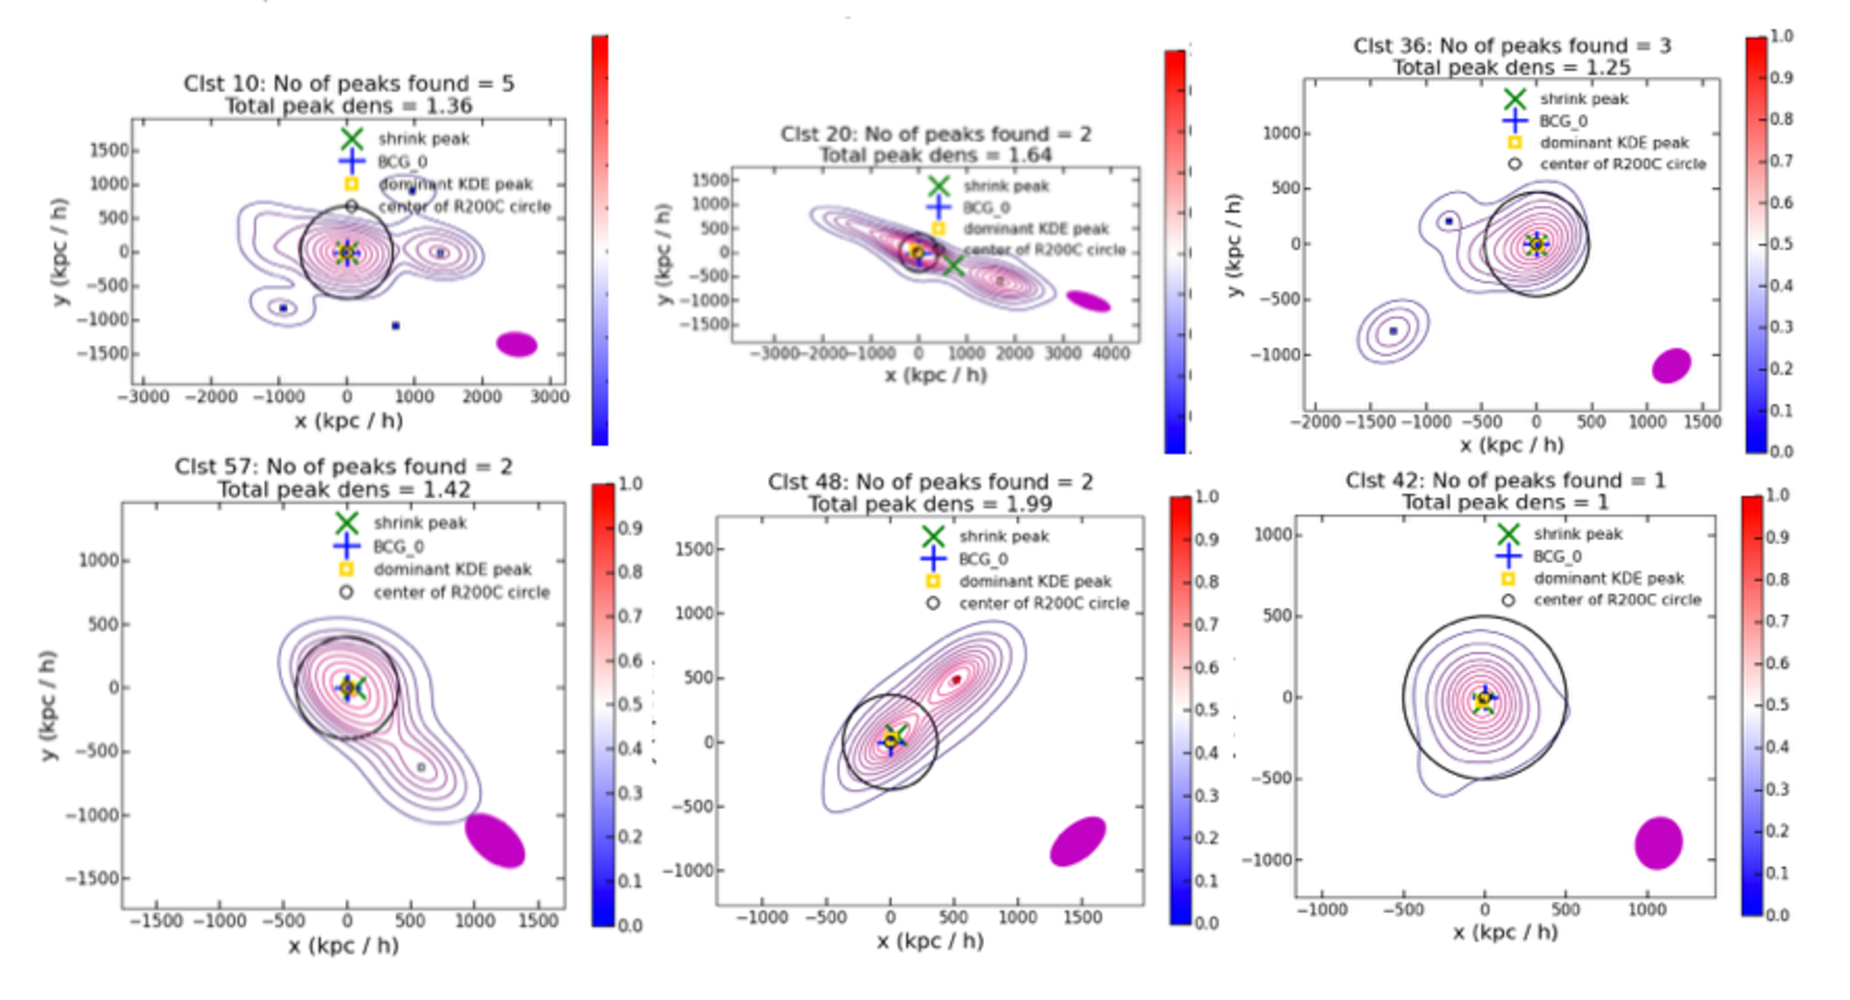
\includegraphics[width=.95\linewidth]{ph_fig_galaxycenter_IllustrisClusters.pdf}
	% 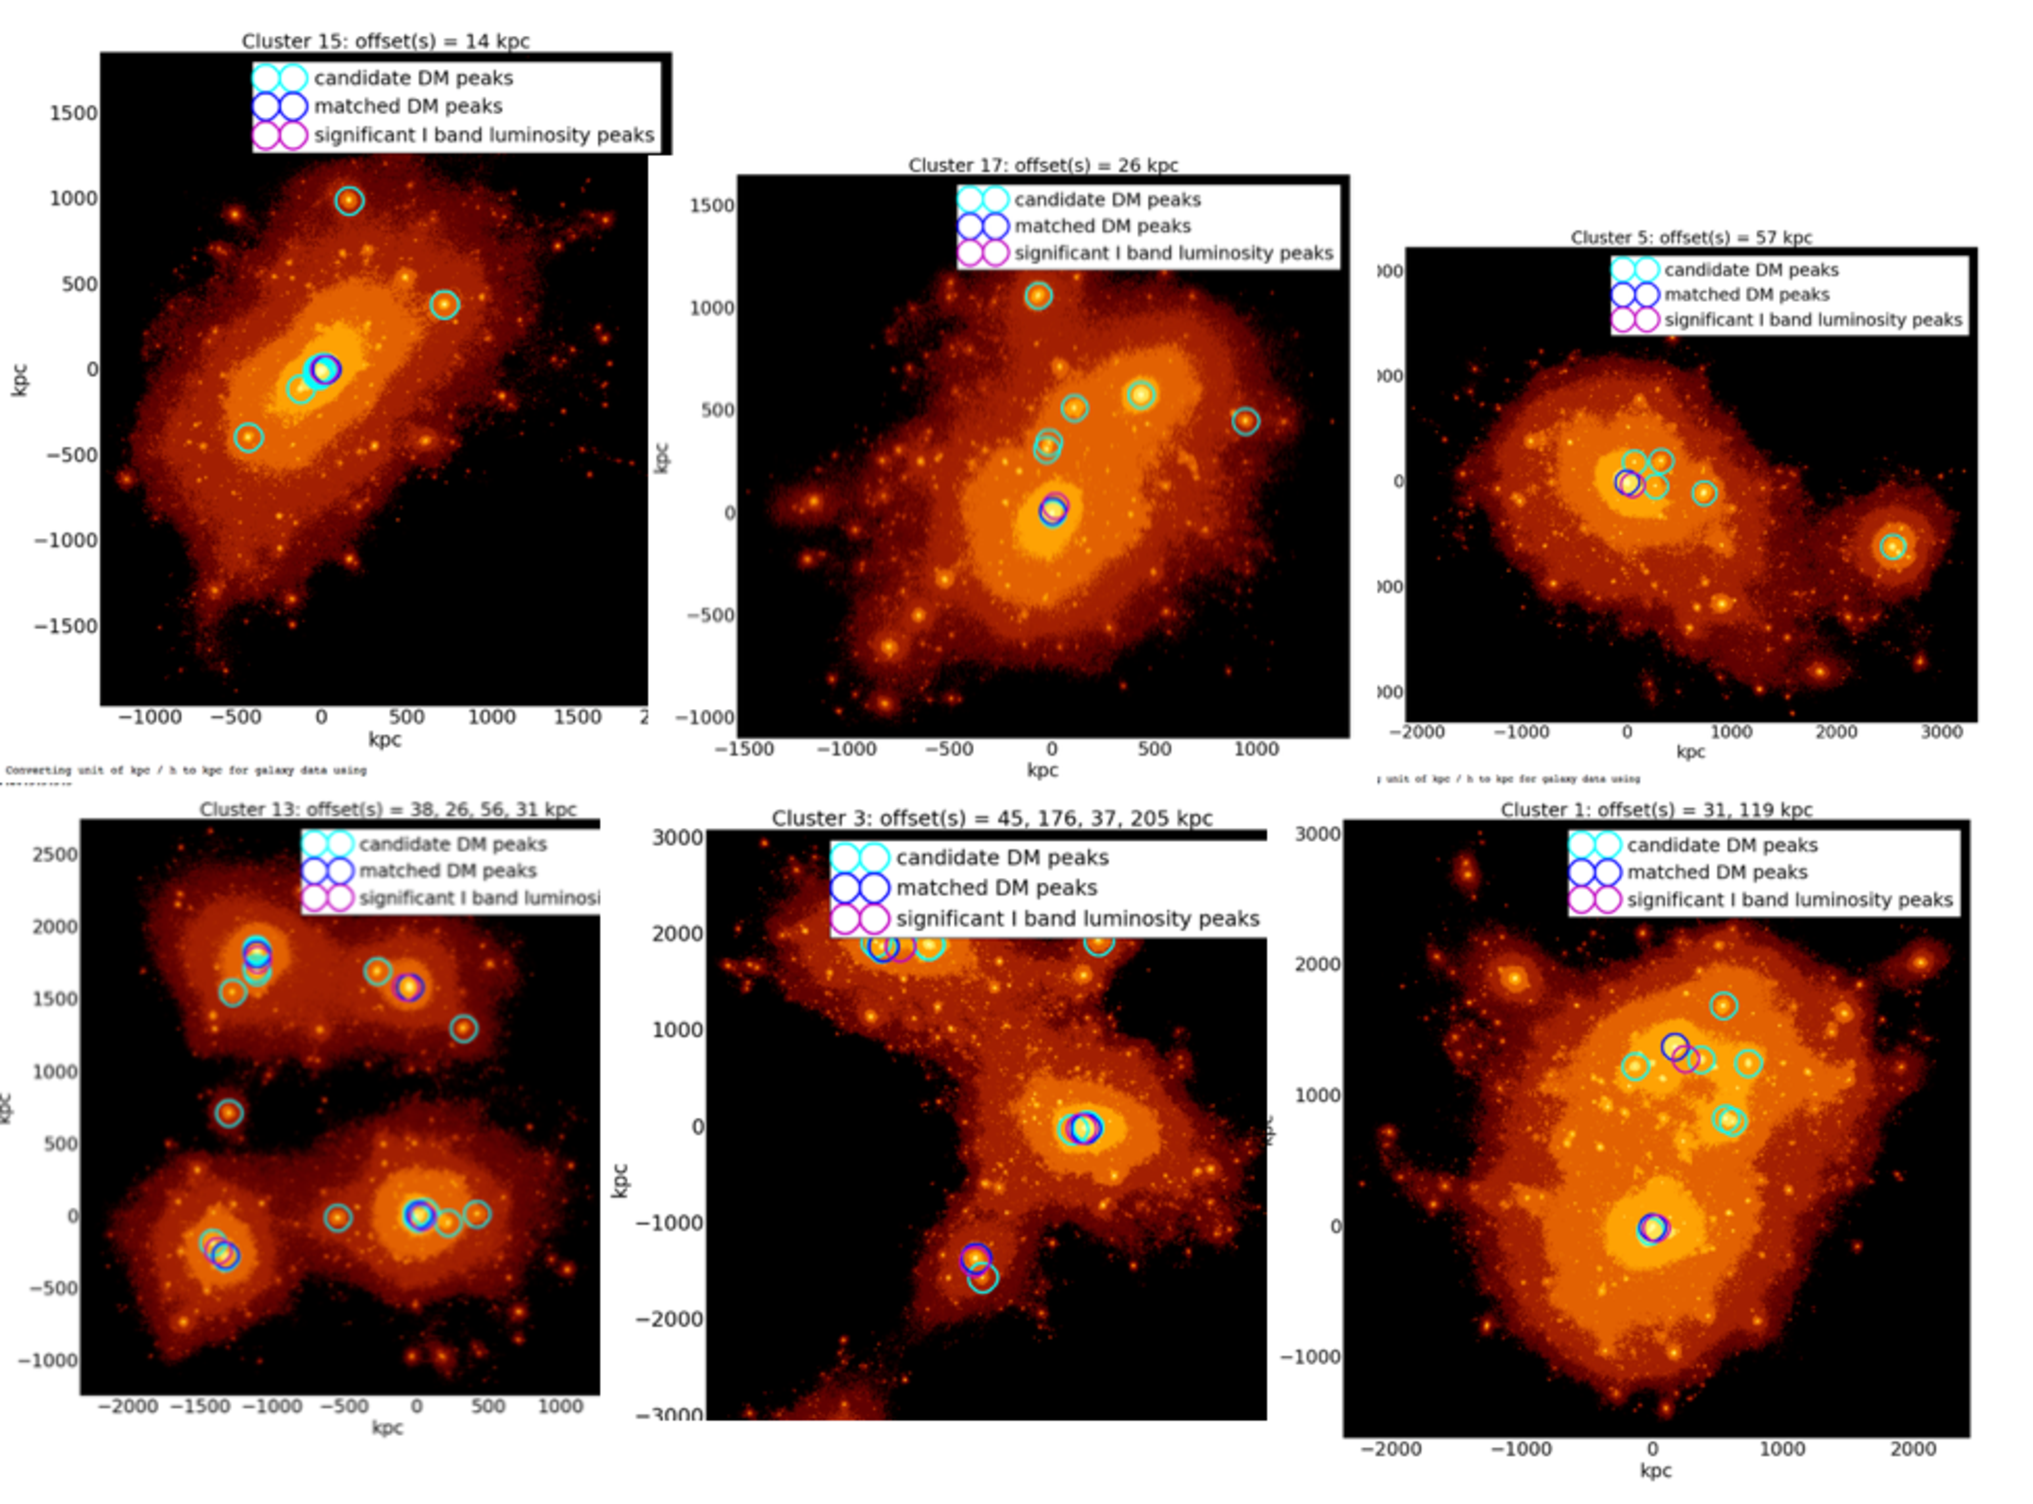
\includegraphics[width=.95\linewidth]{ph_fig_DMcenter_IllustrisClusters.pdf}
	\caption{ {\bf Left figure:} Projected density distribution of DM	
		particle data (density overlay). 
		The identified density peaks are indicated by colored circles. 
		{\bf Right figure:} Projected kernel density estimates (KDE) of member
		galaxies of the same clusters. The projections of the clusters are  
		selected at random.		
		\label{fig:select_peak_visualization}
	}
\end{figure*}


\subsection{Smoothness of dark matter distribution}
From the plots with peak identification, it can be shown that most clusters are
multiply peaked. The actual location of these peaks also depend sensitively 
on the lensing kernel size and the exact reconstruction method.  
Ill-defined problem without a unique solution 

\subsection{Miscentering?}


\subsection{Galaxy-DM Offset in Illustris}
\subsubsection{Projected offsets}
\begin{itemize}
\item those between BCG, the most bound particle and the other masses. 
\item explain the variation of the offsets for the same cluster under different 
projections 
\end{itemize}

% \begin{figure*}
% 	% \includegraphics[width=.95\linewidth]{distribution_of_offsets.eps}
% 	\caption{The probability distribution of the estimated offsets between 
% 		different summary statistics over 43 selected clusters for DM with 2 kpc 
% 		resolution.  
% 
% 		\label{fig:est_offset_distrib_for_different_clusters_2kpc_resolution}}
% \end{figure*}
% 
% \begin{figure*}
% 	\caption{
% 		The probability distribution of the estimated offsets between different
% 		summary statistics over 43 selected clusters for DM with 50 kpc 
% 		resolution.  
% 
% 		\label{fig:est_offset_distrib_for_different_clusters_50kpc_resolution}}
% \end{figure*}
% 
% \begin{figure*}
% 	% \includegraphics[width=.95\linewidth]{distribution_of_offsets.eps}
% 	\caption{The probability distribution of the estimated offsets for different
% 		projections.
% 		\label{fig:est_offset_distrib_for_different_projections}}
% \end{figure*}

\subsubsection{Correlations between the offsets and properties of the cluster / groups}
\begin{itemize}
\item relaxedness
\item mass 
\item richness  
\end{itemize}


\section{DISCUSSION}



\label{sec:discussion}
\subsection{Comparison to other simulations}
\subsection{Comparison to other observational studies}
Central galaxy paradigm (CGP)


% As there are no well-established procedure for summarizing the peak or the
% center of a cluster, nor there is a good m 
There are many aspects of the analysis that is not covered by this study that
are performed for analyzing observational data, such as 

\begin{itemize}
		\item galaxy membership identification along the line of sight
		\item removal of foreground galaxies  
	\end{itemize}
	that are important for calculating the $\sigma_{\rm SIDM}$ with using a
	galaxy-DM offset. 


\subsection{Galaxy-DM Offset in Merging Galaxy Clusters}

\section{SUMMARY}
We showed that 
\begin{itemize}
		\item  the peak finding method To-be-finalized for the density of cluster
			galaxies is the least biased due to substructures from our test data. 
		\item  all existing peak finding methods have non-negligible uncertainty 
			due to the small number of data points. When dealing with small number of
			cluster samples, the uncertainties of the peak locations should not be
			ignored.
		\item the resolution of the DM distribution can / cannot affect
			$\Delta s$.   
		\item the large number of decisions that goes into computing the offsets
			from simulations make it hard if not impossible for comparison between studies. 
			We call researchers in this field to make their software and analysis code openly
			available.
\end{itemize}




\section{ACKNOWLEDGEMENTS}
Our software setup is available through a Docker image on DockerHub while the
main code are version controlled via Git and GitHub. 
Part of the work before the conception of this paper was discussed during 
the AstroHack week 2014. KN would like to thank Phil
Marshall and Jake Vanderplas for preliminary discussions for analyzing galaxy clusters. 
Part of this work was performed under HST grant (TODO ask Dave for grant
number). 



% alternative ways of characterizing differences between DM and galaxy
% distributions.

% \section{The Physical properties of a galaxy cluster}
% State variables are missing.
% A galaxy cluster is not a closed system. 

% correct for multiple comparisons
% High number of latent variables 
% have to rule out the possibility that observables of SIDM being affected by
% the merger history of the cluster. 


